%%%%%%%%%%%%%%%%%%%%%%%%%%% asme2e.tex %%%%%%%%%%%%%%%%%%%%%%%%%%%%%%%
% Template for producing ASME-format articles using LaTeX            %
% Written by   Harry H. Cheng                                        %
%              Integration Engineering Laboratory                    %
%              Department of Mechanical and Aeronautical Engineering %
%              University of California                              %
%              Davis, CA 95616                                       %
%              Tel: (530) 752-5020 (office)                          %
%                   (530) 752-1028 (lab)                             %
%              Fax: (530) 752-4158                                   %
%              Email: hhcheng@ucdavis.edu                            %
%              WWW:   http://iel.ucdavis.edu/people/cheng.html       %
%              May 7, 1994                                           %
% Modified: February 16, 2001 by Harry H. Cheng                      %
% Modified: January  01, 2003 by Geoffrey R. Shiflett                %
% Use at your own risk, send complaints to /dev/null                 %
%%%%%%%%%%%%%%%%%%%%%%%%%%%%%%%%%%%%%%%%%%%%%%%%%%%%%%%%%%%%%%%%%%%%%%

%%% use twocolumn and 10pt options with the asme2e format
\documentclass[twocolumn,10pt]{asme2e}
\special{papersize=8.5in,11in}
\usepackage{graphicx,amsmath,amssymb,mathtools,xcolor}

%% The class has several options
%  onecolumn/twocolumn - format for one or two columns per page
%  10pt/11pt/12pt - use 10, 11, or 12 point font
%  oneside/twoside - format for oneside/twosided printing
%  final/draft - format for final/draft copy
%  cleanfoot - take out copyright info in footer leave page number
%  cleanhead - take out the conference banner on the title page
%  titlepage/notitlepage - put in titlepage or leave out titlepage
%  
%% The default is oneside, onecolumn, 10pt, final

%%% Replace here with information related to your conference
\confshortname{IMECE 2022}
\conffullname{the ASME 2021 International Mechanical Engineering Congress \& Exposition}

%%%%% for date in a single month, use
%\confdate{24-28}
%\confmonth{September}
%%%%% for date across two months, use
\confdate{October 30- November 3}
\confyear{2022}
\confcity{Columbus, Ohio}
\confcountry{USA}

%%% Replace DETC2009/MESA-12345 with the number supplied to you 
%%% by ASME for your paper.
\papernum{IMECE2022-95466}

%%% You need to remove 'DRAFT: ' in the title for the final submitted version.
\title{DRAFT: Sliding Mode Control of a Quad-Copter for Autonomous Trajectory Tracking }
%%% for the discussion section only
%\usepackage{helvet}
%\title{\fontfamily{phv}\selectfont{\Huge{DRAFT: AN ARTICLE CREATED USING \LaTeX2\raisebox{-.3ex}{$\epsilon$}\ IN ASME FORMAT}}}

%%% first author
\author{Daniel Wood
	\affiliation{Mechatronics and Robotics Laboratory\\
		Department of Mechanical aEngineering\\
		North Dakota State University\\
		Fargo, ND 58102\\
		Email: daniel.wood@ndsu.edu
	}	
}

%%% second author
%%% remove the following entry for single author papers
%%% add more entries for additional authors
\author{Majura F. Selekwa\thanks{Address all correspondence to this author.} 
	\affiliation{Mechatronics and Robotics Laboratory\\
		Department of Mechanical aEngineering\\
		North Dakota State University\\
		Fargo, ND 58102\\
		Email: majura.selekwa@ndsu.edu
	}
}

\begin{document}
\maketitle
\begin{abstract}
	{\it  Unmanned air vehicles or drones have become ubiquitous in our daily lives; they are deployed in performing many tasks from dangerous military missions to simple recreation activities. One air vehicle that has become very popular is the quad-copter driven by four vertical and parallel propellers. Today quad-copters are deployed in many video recording and remote monitoring almost everywhere in the world. One area of interest for quad-copters has been in farming operations; these vehicles are used in farming operations for not only aerial monitoring of soil nitrogen levels but many other farm monitoring operations. One common aspect of most quad-copters is that they are teleoperated by the user, i.e., most of them are not yet fully autonomous. There must be a remote pilot who is connected to the quad-copter by a video link so that he/she can control the maneuver of the vehicle along the intended path. This paper intends to show that a quad-copter can be programmed to run autonomously along a predetermined trajectory by using sliding mode control strategy. Since trajectories in most farms are clearly well known in advance, then they can be programmed into the controller for the quad-copter to autonomously track. The design process involves using the intended trajectory to define the 3-D sliding surface and then letting the quad-copter controller switch about that surface while keeping the vehicle in the target trajectory. The workspace is defined as a 3-D space where the sliding surface is defined by fitting weighted spline functions on the coordinates of the intended trajectory to define the stable sliding surface whose stability lever increases as the vehicle moves towards the target point. Preliminary results compare the trajectories followed by the quad-copter and the intended trajectories by using the mean square deviation. As would be expected, the performance depends heavily on the speed of the quad-copter; higher speeds on sharp curvature are associated with large tracking errors than low speeds on similar curvatures, while the performance on straight line paths was considerably good. This is  most likely due to the switching speed because it seems that higher speeds should be associated with higher switching speeds also. The future work intends to study if parameterizing the 3-D splines using speed and time can improve the tracking performance where the switching rate will be made to be proportional to the number of spline functions that define the trajectory irrespective of the speed of the quad-copter.
	}\end{abstract}

\section{Introduction}
{\color{blue}
In recent years the development of smaller and cheaper electronics, specifically inertial measurement systems, has led to a rise in popularity of lightweight unmanned aerial vehicles. Unmanned aerial vehicles come in many configurations, some of the more common are quadrotors, octocopters as well as single engine. This work in particular will focus entirely on the quadrotor configuration. 

The increase in general usage of quadrotor vehicles, has led to the need to autonomously control these vehicles, some applications include automated delivery services, military usage, aerial imagery. In recent years companies have begun implementing tethering features that allow quadrotors to autonomously follow a target. More sophisticated systems utilize autonomous path tracking. This path tracking is realized through a robust control scheme.

The formation of autonomous control consists of a valid dynamical model of the vehicle, and a fast, stable, robust controller. The dynamics of a quadrotor is not trivial and requires concepts from advanced dynamics topics. There are many control algorithms to choose from, some that are currently being utilized. Picking a control algorithm stems from the goal of making the output stable as well as having a robust controller. A system is said to be stable if it can remain at an equilibrium point under the stress of external disturbances [cite something ehre], whereas robustness is defined as a controller that can operate under parameters that vary from the original design [ cite something here].

There are many researchers dedicating time to improving controller stability through different control schemes such as Multiple Input Multiple Output state variable (MIMO) \cite{FarameeVeeravat2014EotS}, Linear Quadratic Regulator (LQR), Model Predictive Control (MPC), and Sliding Mode Control (SMC). In general this research focuses on nuances of the choosen algorithm with the goal of improvement in disturbance rejection\cite{DenisKotarski2016CDFU} and robustness. Because of the scope of the research, the dynamics model of the quadrotor is generally linearized for simplicity, or assumptions that were made lead to reduced order of the system\cite{FarameeVeeravat2014EotS}. Higher order dynamics that are missed when a model is linearized can contribute to errors in the control scheme. 

The goal of this research is to start with the concrete fundamentals of dynamics to derive a state space model of the quadrotor in 3D space, relative to a fixed global frame. Then create a stable and robust non-linear controller for accurate path tracking. This controller will be based on the Sliding Mode Control (SMC) method, which is a specific type of variable structure system. This method is a valid choice for this dynamical system because it allows the controller to quickly jump to different equilibrium points, and forces state variables towards the equilibrium points, or in the case of SMC, the sliding manifold as it is noted in literature.

Derivation of the equations of motion of the quadrotor requires defining two coordinate systems, the global, or fixed frame, and the body, or inertial frame\cite{FanniMohamed2017AN6Q},\cite{FarameeVeeravat2014EotS},\cite{HaomiaoHuang2009Aaco},\cite{DenisKotarski2016CDFU}. The path that is defined is always given in reference to the global frame, whereas the equations of motion that define our controllable states, is in reference to the body frame. Rotations of the body such as yaw, pitch, roll, are determined through sensors such as accelerometers and IMUs physically placed on the body. While physical position in space is defined by a global positioning system (GPS), which requires knowledge of the body as well as the reference frame.

Sliding mode control is a technique that allows}

\section*{QUADCOPTER MODELLING}
%\subsection*{The Dynamic Model}
In order to control the quadcopter, its clear dynamic model is needed. The quadcopter model uses a mix of vehicle's body frame $(x,y,z) $ through which it reads its sensors, but its motion is controlled using the global inertial frame $(X,Y,Z)$, so the sensor readings of the quadcopter must always be translated by the controller back into these global coordinates. Currently, there are two dynamic models that are popular among researchers on quadcopters: the most popular one is the  model of \cite{1013341}, which is a system of simplified Newton-Euler equations where the Newton equations are taken in the global frame, and the Euler equations are taken in the body frame using Euler rates. This model has been the most popular among quadcopter researchers as recently as \cite{lee2009feedback,mu2019learning,castillo2019disturbance}. The next model is that of \cite{bouabdallah2007design}, which also has been very popular among researchers, see for example \cite{mellinger2012trajectory,alexis2011switching,leishman2014quadrotors}. The model of  \cite{bouabdallah2007design} is based on Lagrangian formalism assuming that the cosines and sines of Euler angles for the rotation part of the motion are negligible except for the linear part of the motion. Both the models of \cite{1013341} and \cite{bouabdallah2007design} assume that the quadcopter measurements represent the state vector, i.e., the 3-D coordinates of the vehicle, the three Euler angles and their rates of change. There are some applications where this assumption is not realizable, even with quadcopters equipped with high precision GNSS device, because most onboard gyrometers can only measure angular velocities, not Euler rates.


This section develops a model also using Lagrangian formalism but limits cases where the Euler angles can be ignored. On the rotary part of the motion, the model uses angular velocities of the vehicle, which can be measured by its gryometers instead of  the Euler rates.
\begin{figure}[h]
	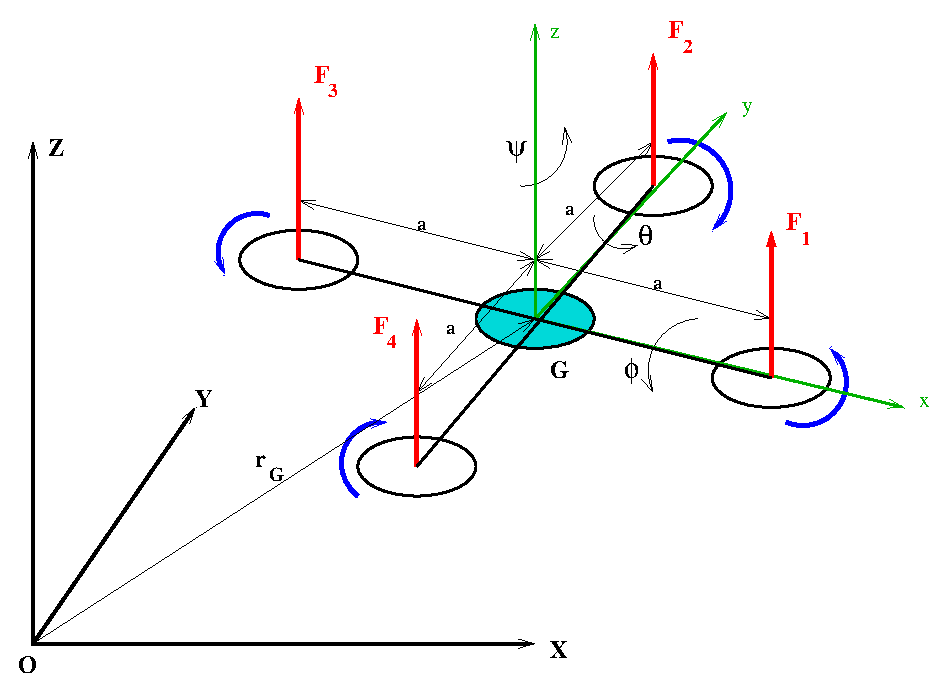
\includegraphics[scale = 0.5]{model.eps}
	\caption{Free Body Diagram of Quadcopter}
\end{figure}

If the position of the quadcopetr in the global frame is  defined by coordinates ($X_G, Y_{G}, Z_{G})$ and the orientation of its body frame $(x,y,z)$ in the global frame is  defined by Euler  angles ($\psi,\theta,\phi$), then  its generalized coordinates  become
\begin{equation}
q=[\begin{array}{cccccc}
X_{G} & Y_{G} & Z_{G} & \psi & \theta & \phi\end{array}]^T= [\begin{array}{cccccc}
q_{1} & q_{2} & q_{3} & q_4 & q_5 & q_6\end{array}]^T
\end{equation}

The transformation form the body frame to global frame is implemented through a rotation matrix
{\small
\begin{align}
	R^b_G=&
	\left[\begin{array}{ccc} \cos{q_{4}}\cos{q_{5}} &~ \cos{q_{4}}\sin{q_{5}}\sin{q_{6}}-\cos{q_{6}}\sin{q_{4}} & \\ 
		\cos{q_{5}}\sin{q_{4}} & ~\cos{q_{4}}\cos{q_{6}}+\sin{q_{4}}\sin{q_{5}}\sin{q_{6}} & \cdots\\ 
		-\sin{q_{5}} & ~\cos{q_{5}}\sin{q_{6}} &  \end{array}\right.\notag\\
&\qquad	
\left.\begin{array}{cc}
&\sin{q_{4}}\sin{q_{6}}+\cos{q_{4}}\cos{q_{6}}\sin{q_{5}}\\
\cdots&\cos{q_{6}}\sin{q_{4}}\sin{q_{5}}-\cos{q_{4}}\sin{q_{6}}\\
&\cos{q_{5}}\cos{q_{6}}\end{array}\right]
\end{align}
Let the four forces produced by the thrust propellers in the body frame be
\begin{equation}
\vec{F}_{i}^b=\left[\begin{array}{ccc}
	0&\quad
	0&\quad
	F_{i}
\end{array}\right]^T,\qquad i=1,2,3,4,
\end{equation}
all acting at a distance $a$ from the center of gravity $G$ with $F_1$ and $F_3$ acting on the $x$- axis and $F_2$ and $F_4$ acting on the $y$-axis. Then the resultant moments of these forces about the quadcopters center of gravity in the body frame becomes 
\begin{equation}
	\vec{M}^b_G=\left[\begin{array}{ccc}
		a\left(F_{2}-F_{4}\right)&\quad
		-a\left(F_{1}-F_{3}\right)&\quad
		0
	\end{array}\right]^T
\end{equation}
of all forces acting on the quadcopter in the global frame becomes
\begin{equation}
\vec{F}_{R}(q)=\left[\begin{array}{c}
	(F_{1}+F_{2}+F_{3}+F_{4})\left(\cos q_4 \sin q_5 \cos q_6+\sin q_4\sin q_6\right)\\
	(F_{1}+F_{2}+F_{3}+F_{4})\left(\sin q_4 \sin q_5 \cos q_6-\cos q_4\sin q_6\right)\\
	\left(F_{1}+F_{2}+F_{3}+F_{4}\right)\cos q_{5}\cos q_{6}-W
\end{array}\right]
\end{equation}
where $W$ is the weight of the vehicle. 

%And the resultant moment of these forces about $G$ become
%
%{\small
%\begin{equation}
%	\vec{M}_{G}(q)=a\left[\begin{array}{c}
%		(F_{1}-F_{4})\cos q_4\cos q_5+\cdots\\
%		\quad\cdots (F_2-F_3)(\cos q_4\sin q_5\sin q_6-\sin q_4\cos  q_6)\\
%		\\
%		(F_{1}-F_{4})\sin q_4\cos q_5+\cdots\\
%		\quad\cdots (F_2-F_3)(\sin q_4\sin q_5\sin q_6+\cos q_4\cos  q_6)\\
%		\\
%		-(F_{1}-F_{4})\sin q_5+ (F_2-F_3)\cos q_5\sin q_6\\
%	\end{array}\right]
%\end{equation}}


 If $\dot{q}_5, \dot{q}_6,$ and $\dot{q}_7$ are the yaw, pitch and roll rates (or Euler rates)  of the vehicle, then its angular velocity in the body frame becomes
 
 \begin{equation}
 	\vec{\omega}^b=\left[\begin{array}{c}
 		\omega_{x}\\
 		\omega_{x}\\
 		\omega_{x}
 	\end{array}\right]=\left[\begin{array}{ccc} -\sin{q}_{5} & 0 & 1\\ \cos{q}_{5}\sin{q}_{6} & \cos{q}_{6} & 0\\ \cos{q}_{5}\cos{q}_{6}) &-\sin{q}_{6} & 0 \end{array}\right]\end{equation}
Since the position vector of $G$ in the inertial frame is 
\begin{equation}
	\vec{r}_{G}= \left[\begin{array}{ccc}
		q_1&\quad
		q_2&\quad
		q_3
	\end{array}\right]^T
\end{equation}
then the generalized forces $Q_{i}$ acting on the vehicle can be defined  as
\begin{equation}
Q_{i}=\vec{F}_{R}\cdot\frac{\partial\vec{r}_{G}}{\partial q_{i}}+\vec{M}_{G}^b\frac{\partial\vec{\omega}^b}{\partial\dot{q_{i}}}, \qquad \forall i=1,2\cdots, 6,\end{equation}
and the generalized mass of the vehicle can also be defined as
\begin{equation}
M(q)=\left(\frac{\partial\vec{r}_{G}}{\partial q}\right)^{T}m_{rr}\frac{\partial\vec{r}_{G}}{\partial q}+\left(\frac{\partial\vec{\omega}^b}{\partial\dot{q}}\right)^{T}m_{\theta\theta}\frac{\partial\vec{\omega}^b}{\partial\dot{q}}
\end{equation}

with

\begin{equation}
m_{rr}=\left[\begin{array}{ccc}
	m & 0 & 0\\
	0 & m & 0\\
	0 & 0 & m
\end{array}\right],\qquad
m_{\theta\theta}=\left[\begin{array}{ccc}
	I_{xx} & 0 & 0\\
	0 & I_{yy} & 0\\
	0 & 0 & I_{zz}
\end{array}\right]
\end{equation}

It is from these quantities that equations of motion for the quad-copter can be established by
\begin{equation}
\frac{d}{dt}\left(\frac{\partial T(q,\dot{q})}{\partial\dot{q_{j}}}\right)-\frac{\partial T(q,\dot{q})}{\partial q_{j}}=Q_{j}(q)\label{eqL}
\end{equation}
 where $T$ is the kinetic energy  expressed  by
\begin{equation}
T(q,\dot{q})=\frac{1}{2}\dot{q}^{T}M(q)\dot{q}
\end{equation}
%
%\[T= \frac{m\dot{q}_{1}^2}{2}+\frac{m\dot{q}_{2}^2}{2}+\frac{m\dot{q}_{3}^2}{2}+\frac{I_{x}{\dot{q}_{6}}^2}{2}+\frac{I_{y}{\dot{q}_{5}}^2}{2}+\frac{I_{x}\dot{q}_{4}^2\sin^2q_{5}}{2}\cdots\]
%\[-\frac{I_{y}\dot{q}_{5}^2\sin^2q_{6}}{2}+\frac{I_{z}\dot{q}_{5}^2\sin^2q_{6}}{2}+\frac{I_{z}\dot{q}_{4}^2\cos^2q_{5}\cos^2q_{6}}{2}\cdots\]
%\[+\frac{I_{y}\dot{q}_{4}^2\cos^2{q}_{5}\sin^2q_{6}}{2}-I_{x}\dot{q}_{4}\dot{q}_{6}\sin{q}_{5}\cdots\]
%\[+I_{y}\cos{q}_{5}\cos{q}_{6}\sin{q}_{6}\dot{q}_{4}\dot{q}_{5}\cdots\]
%\[-I_{z}\cos{q}_{5}\cos{q}_{6}\sin{q}_{6}\dot{q}_{4}\dot{q}_{5} \]

%\[T= \tfrac{1}{2}m\dot{q}_{1}^2+\tfrac{1}{2}m\dot{q}_{2}^2+\tfrac{1}{2}m\dot{q}_{3}^2+\tfrac{1}{2}I_{x}{\dot{q}_{6}}^2+\tfrac{1}{2}I_{y}{\dot{q}_{5}}^2+\tfrac{1}{2}I_{x}\dot{q}_{4}^2\sin^2q_{5}\cdots\]
%\[+\tfrac{1}{2}(I_{z}-I_y)\dot{q}_{5}^2\sin^2q_{6}+\tfrac{1}{2}I_{z}\dot{q}_{4}^2\cos^2q_{5}\cos^2q_{6}+\tfrac{1}{2}I_{y}\dot{q}_{4}^2\cos^2{q}_{5}\sin^2q_{6}\cdots\]
%\[-(I_{z}-I_y)\dot{q}_{4}\dot{q}_{5}\cos{q}_{5}\cos{q}_{6}\sin{q}_{6}-I_{x}\dot{q}_{4}\dot{q}_{6}\sin{q}_{5} \]
%%Although it is known that $I_{xx}\ne I_{yy}\ne I_{zz}$, equation (\ref{eqL})  is simplified by assuming that $I_{xx}\approx  I_{yy}$ in particular because of the geometry of most quadcopters. 
The development in this work assumes that the values of Euler angles are bound within the range from $-\tfrac{\pi}{6}\le\left(\psi,\theta,\phi\right)\le \tfrac{\pi}{6};$ therefore higher orders of sine terms can be ignored. The resulting kinetic energy leads to the following equations of motion:
%\begin{align}T=& \tfrac{1}{2}m\dot{q}_{1}^2+\tfrac{1}{2}m\dot{q}_{2}^2+\tfrac{1}{2}m\dot{q}_{3}^2+\tfrac{1}{2}I_{x}{\dot{q}_{6}}^2+\tfrac{1}{2}I_{y}{\dot{q}_{5}}^2+\tfrac{1}{2}I_{z}\dot{q}_{4}^2\cdots\notag\\
%&\qquad\cdots-(I_{z}-I_y)\dot{q}_{4}\dot{q}_{5}\cos{q}_{5}\cos{q}_{6}\sin{q}_{6}-I_{x}\dot{q}_{4}\dot{q}_{6}\sin{q}_{5} \end{align}
\begin{align}
&\ddot{q}_{1}=\tfrac{1}{m}(F_{1}+F_{2}+F_{3}+F_{4})\cos q_4 \sin q_5 \cos q_6\label{eom1}\\
&\ddot{q_{2}}=-\tfrac{1}{m}(F_{1}+F_{2}+F_{3}+F_{4})\cos q_4\sin q_6\\
&\ddot{q_{3}}=\tfrac{1}{m}(F_{1}+F_{2}+F_{3}+F_{4})\cos q_{5}\cos q_{6}-\tfrac{W}{m}\\
& I_{z}\ddot{q}_{4}-(I_z-I_{x})\ddot{q}_{5}\cos{q}_{5}\cos{q}_{6}\sin{q}_{6}-(I_z-I_y+I_x)\dot{q}_5\dot{q}_6\cos{q}_5\cdots\notag\\
&\qquad\cdots-I_{x}\ddot{q_{6}}\sin{q}_{5}=	a(F_{4}-F_{2})\sin q_5+ a(F_3-F_1)\cos q_5\sin q_6\\
&I_x\ddot{q}_5-(I_z-I_{x})\ddot{q}_{4}\cos{q}_{5}\cos{q}_{6}\sin{q}_{6}-(I_z-2I_{x})\dot{q}_{4}\dot{q}_{6}\cos{q}_{5}\cdots\notag\\
&\qquad\cdots=a(F_3-F_1)\cos q_6\\
&I_x\ddot{q}_6-I_{x}\ddot{q}_4\sin q_5+(I_z-I_y-I_x)\dot{q}_4\dot{q}_5\cos{q}_5=-a(F_{4}-F_2)\label{eom6}
\end{align}

Now, if a state vector is defined as
\begin{equation}
	\textbf{x}= \left[\begin{array}{cc}
		q&\quad
		\dot{q}
	\end{array}\right]^T
\end{equation}
and the control input is 
\begin{equation}
	\textbf{u}= \left[\begin{array}{cccc}
		F_1&\quad
		F_2&\quad
		F_3&\quad
		F_4
	\end{array}\right]^T
\end{equation}
then the equations of motion (\ref{eom1})-(\ref{eom6}) can be expressed in state space form as
\begin{equation}
\dot{\textbf{x}}=\textbf{f}(\textbf{x})+\textbf{g}(\textbf{x})\textbf{u}+\textbf{W}\label{eqssM}
\end{equation}
Reverting to the notation of a stat vector $X\in\mathbb{R}^{12}$ instead of the generalized coordinate $q$ we define 
\begin{align}
	\alpha_1(\textbf{x})&=\tfrac{1}{m}\cos x_4 \sin x_5 \cos x_6\\
	\alpha_2(\textbf{x})&=-\tfrac{1}{m}\cos x_4\sin x_6\\
	\alpha_3(\textbf{x})&=\tfrac{1}{m}\cos x_{5}\cos x_{6}
\end{align}
so that
\begin{equation}
	\textbf{f}(\textbf{x})=\left[\begin{array}{c}
		x_7\\
	x_8\\
		x_9\\
		x_{10}\\
		x_{11}\\
	x_{12}\\
	0\\
	0\\
	0\\ \frac{I_y}{I_z}x_{10}x_{11}\cos{x}_{5}\sin{x}_{5}+\left(\frac{I_{x}-I_y+I_z}{I_z}\right)x_{11}x_{12}\cos{x}_{5}\cdots\\\qquad\cdots+\left(\frac{2{I_{x}}^2+{I_{z}}^2-3\,I_{x}I_{z}}{I_xI_z}\right)x_{10}x_{12}\cos{x}_{6}\sin{x}_{6}\\
	\left(\frac{I_z-2I_x}{I_x}\right)x_{10}x_{11}\cos{x}_{5}+\left(\frac{(I_z-I_x)(I_x-I_y+I_z)}{I_xI_z}\right)x_{11}x_{12}\cos{x}_{6}\sin{x}_{6}\\
	\frac{I_y}{I_x}x_{10}x_{11}\cos{x}_{5}+\left(\frac{I_{x}-I_y+I_z}{I_z}\right)x_{11}x_{12}\cos{x}_{5}\sin{x}_{5}
	\end{array}\right]
\end{equation}
and
{\scriptsize\begin{equation}
\textbf{g}(\textbf{x})=\left[\begin{array}{cccc}
	0\quad&0\quad&0\quad&0\\
	0\quad&0\quad&0\quad&0\\
	0\quad&0\quad&0\quad&0\\
	0\quad&0\quad&0\quad&0\\
	0\quad&0\quad&0\quad&0\\
	0\quad&0\quad&0\quad&0\\
	\alpha_1(\textbf{x})\quad&\alpha_1(\textbf{x})\quad&\alpha_1(\textbf{x})\quad&\alpha_1(\textbf{x})\\
	\alpha_2(\textbf{x})\quad&\alpha_2(\textbf{x})\quad&\alpha_2(\textbf{x})\quad&\alpha_2(\textbf{x})\\
	\alpha_3(\textbf{x})\quad&\alpha_3(\textbf{x})\quad&\alpha_3(\textbf{x})\quad&\alpha_2(\textbf{x})\\
	\tfrac{a}{I_x}\cos x_5\sin{x_6}&0&-\tfrac{a}{I_x}\cos x_5\sin{x_6}&0\\
	-\tfrac{a}{I_x}\cos x_6&0&\tfrac{a}{I_x}\cos x_6&0\\
	0&\tfrac{a}{I_x}&0&-\tfrac{a}{I_x}
\end{array}\right]
\end{equation}}
where \textbf{W} is a constant vector contributed by gravity $g$ defined in this case as
{\scriptsize\begin{equation}
	\textbf{W}=\left[\begin{array}{c}
	0\\
	0\\
	0\\
	0\\
	0\\
	0\\
	0\\
	0\\
	-g\\
	0\\
	0\\
	0
	\end{array}\right]
	\end{equation}}

Then it turns out that any nonlinear control that can control the system of (\ref{eqssM}) can also be applied on this vehicle. The next section suggests implementing a sliding mode control structure for tracking a predetermined path $\textbf{p}(t)$.

\section*{CONTROL STRUCTURE}
The quadcopter is assumed to be equipped with an RTK GPS, a gyrometer, and a baromteric pressure altmeter. Useful measurements $\textbf{y}_m$ are the  $X$ and $Y$ coordinates measured by the GPS in the UTM projection as Eastings and Northings, the altitude $Z$  measured by the barometeric pressure altimeter along with euler rates $\dot{\psi}, \dot{\theta},$ and $\dot{\phi}$ measured from the gyrometer; i.e.,
\begin{equation}\textbf{y}_m=\left[\begin{array}{c}
		X\\
		Y\\
		Z\\
		\dot{\psi}\\ 
		\dot{\theta}\\
		\dot{\phi}
	\end{array}\right]=\left[\begin{array}{c}
		x_1\\
		x_2\\
		x_3\\
		x_{10}\\
		x_{11}\\
		x_{12}
	\end{array}\right]\end{equation}
However, useful measurements $\textbf{y}$ for use in trajectory control  will be the linear positions only, i.e.,
\begin{equation}\textbf{y}=h(\textbf{x})=\left[\begin{array}{c}
	X\\
	Y\\
	Z
\end{array}\right]=\left[\begin{array}{c}
x_1\\
x_2\\
x_3
\end{array}\right]\end{equation}
This is a MIMO nonlinear system  that can be expressed with four inputs as
\begin{align}\dot{\textbf{x}}&=\textbf{f}(\textbf{x})+\textbf{g}(\textbf{x})\textbf{u}=\textbf{f}(\textbf{x})+\sum_{k=1}^4 g_k(\textbf{x})u_k\end{align}
and 3 outputs 
\begin{align}
y_1 &= h_1(\textbf{x})=x_1,\\
y_2 &= h_2(\textbf{x})=x_2,\\
y_3 &= h_3(\textbf{x})=x_3\end{align}
Therefore
\begin{equation}\dot{\textbf{y}}=\textbf{L}_fh(x)+\textbf{L}_{g}h(x)\textbf{u}=\left[\begin{array}{c}
	x_7\\
	x_8\\
	x_9
\end{array}\right]+\left[\begin{array}{cccc}
0&0&0&0\\
0&0&0&0\\
0&0&0&0
\end{array}\right]\left[\begin{array}{c}
u_1\\
u_2\\
u_3\\
u_4
\end{array}\right]
\end{equation}
where $\textbf{L}_\gamma \eta(x)$ is the lie derivative function $\eta(x)$ with respect to function $\gamma(x).$ 
The next derivative lead to
\begin{align}\ddot{\textbf{y}}&=\textbf{L}_f^2h(x)+\textbf{L}_{g}^2h(x)\textbf{u}\label{eq34}\\
	&=\left[\begin{array}{c}
	0\\
	0\\
	0
\end{array}\right]+\left[\begin{array}{cccc}
	\alpha_1(\textbf{x})\quad&\alpha_1(\textbf{x})\quad&\alpha_1(\textbf{x})\quad&\alpha_1(\textbf{x})\\
\alpha_2(\textbf{x})\quad&\alpha_2(\textbf{x})\quad&\alpha_2(\textbf{x})\quad&\alpha_2(\textbf{x})\\
\alpha_3(\textbf{x})\quad&\alpha_3(\textbf{x})\quad&\alpha_3(\textbf{x})\quad&\alpha_2(\textbf{x})\\
\end{array}\right]\left[\begin{array}{c}
u_1\\
u_2\\
u_3\\
u_4
\end{array}\right]
	\end{align}
showing that the system has a relative degree of 1; but its decoupling matrix is singular, therefore direct application of output feedback linearization control will not work \cite{isidori1995nonlinear}. However, this information about the system's relative degree makes it possible to define the sliding surface as\cite{slotine1991applied}
\begin{align}\sigma(\textbf{x},t)&=\left(\frac{d}{dt}+\lambda\right)^1\left[\textbf{y}-\textbf{p}(t)\right]\\
&=\dot{\textbf{y}}-\dot{\textbf{p}}(t)+\lambda\left[\textbf{y}-\textbf{p}(t)\right]\label{eq37}\end{align} 
where $\gamma$ is an arbitrary diagonal matrix  of tolerances allowed on the trajectory error, and $\textbf{p}(t)$ is the desired time dependent trajectory expressed as
\begin{equation}\textbf{p}(t)=\left[\begin{array}{c}
	x_1(t)\\
	x_2(t)\\
	x_3(t)
\end{array}\right],\qquad t\ge0\end{equation}
This sliding surface is independent of the control input $\textbf{u}.$
Now, the Lyapunov function for this motion can be defined in terms of this sliding surface as
\begin{equation}V(\textbf{x})=\tfrac{1}{2}\sigma(\textbf{x},t)^T\sigma(\textbf{x},t)\end{equation}
and for the stability of motion, this function must satisfy the Lyapunov condition
\begin{equation}\dot{V}(\textbf{x},t)=\sigma(\textbf{x},t)^T\dot\sigma(\textbf{x},t)\le0\end{equation}
so that whenever $\sigma(\textbf{x},t)>0$ then $\dot\sigma(\textbf{x},t)<0$ and vice versa. It is from these observations where the sliding control structure can be defined as
\begin{equation}
	\textbf{u}=\begin{cases}
		\begin{array}{lr}
			\textbf{u}^{+}; &  \text{if}\quad \sigma(\textbf{x})>0\\  
			\textbf{u}_o; &  \text{if}\quad \sigma(\textbf{x})=0\\  
			\textbf{u}^{-}; &  \text{if}\quad \sigma(\textbf{x})<0\\
		\end{array}
	\end{cases}\label{eq44}
\end{equation}
where $\textbf{u}_o$ is the control required to drive the quad-copter to the destination while $\textbf{u}^{+}$ and $\textbf{u}^{-}$ are computed to satisfy the corresponding requirements on $\dot\sigma(\textbf{x},t)$ to bring the quad-copter back to the sliding surface.


Equations (\ref{eq34}) and (\ref{eq37}) show that, since $\textbf{L}_f^2h(x)=0$ then by denoting
\begin{equation}\textbf{A}\triangleq\textbf{L}_{g}^2h(x)\end{equation} it follows that
\begin{align}\dot{\sigma}(\textbf{x},t)&=\ddot{\textbf{y}}-\ddot{\textbf{p}}(t)+\lambda\left[\dot{\textbf{y}}-\dot{\textbf{p}}(t)\right]\\
&=\textbf{A}\textbf{u}-\ddot{\textbf{p}}(t)+\lambda\left[\dot{\textbf{y}}-\dot{\textbf{p}}(t)\right]\end{align}
Therefore, $\textbf{u}_o, \textbf{u}^{+}$ and $\textbf{u}^{-}$ must be defined such that
\begin{align}
	\textbf{u}_{+}<\left(\textbf{A}^T\textbf{A}\right)^{-1}\textbf{A}^T\left(\ddot{\textbf{p}}(t)-\lambda\left[\dot{\textbf{y}}-\dot{\textbf{p}}(t)\right]\right), \qquad \sigma(\textbf{x})>0\\
	\textbf{u}_o=\left(\textbf{A}^T\textbf{A}\right)^{-1}\textbf{A}^T\left(\ddot{\textbf{p}}(t)-\lambda\left[\dot{\textbf{y}}-\dot{\textbf{p}}(t)\right]\right), \qquad \sigma(\textbf{x})=0\\
	\textbf{u}_{-}>\left(\textbf{A}^T\textbf{A}\right)^{-1}\textbf{A}^T\left(\ddot{\textbf{p}}(t)-\lambda\left[\dot{\textbf{y}}-\dot{\textbf{p}}(t)\right]\right),\qquad \sigma(\textbf{x})<0 \label{eq46}
\end{align}
For implementation purposes, these equations will be evaluated on element-by-element basis corresponding to the coordinate deviations from the desired path, i.e., \begin{equation}
	\textbf{u}^{(i)}=\begin{cases}
		\begin{array}{lr}
			\textbf{u}_{+}^{(i)}; &  \text{if}\quad \sigma_i(\textbf{x})>0\\  
			\textbf{u}_o^{(i)}; &  \text{if}\quad \sigma_i(\textbf{x})=0\\ 
			\textbf{u}_{-}^{(i)}; &  \text{if}\quad \sigma_i(\textbf{x})<0\\
		\end{array}
	\end{cases},\qquad i=1,2,3
\end{equation}
where for some small smoothing factor $\varepsilon>0$
\begin{align}
	\textbf{u}_{+}^{(i)}&=-\left(\textbf{A}_i^T\textbf{A}_i\right)^{-1}\textbf{A}_i^T\varepsilon\sigma_i(\textbf{x})\\
	\textbf{u}_o^{(i)}&=0\\%\left(\textbf{A}_i^T\textbf{A}_i\right)^{-1}\textbf{A}_i^T\left(\ddot{\textbf{p}}_i(t)-\lambda\left[\dot{\textbf{y}}_i-\dot{\textbf{p}}_i(t)\right]\right)\\
	\textbf{u}_{-}^{(i)}&=\left(\textbf{A}_i^T\textbf{A}_i\right)^{-1}\textbf{A}_i^T\varepsilon\sigma_i(\textbf{x}) \label{eq46}
\end{align}
and $\textbf{A}_i$ is row $i$ of matrix $\textbf{A}$. Since the outer product matrix $\textbf{A}_i^T\textbf{A}_i$ is always singular, the quantity $\left(\textbf{A}_i^T\textbf{A}_i\right)^{-1}\textbf{A}_i^T$ is computed as the Moore-Penrose pseudo inverse of $\textbf{A}_i$ using any convenient numerical algorithm such as the singular value decomposition \cite{strang2006linear}. The overall control signal becomes
\begin{equation}
	\textbf{u}=\left(\textbf{A}^T\textbf{A}\right)^{-1}\textbf{A}^T\left(\ddot{\textbf{p}}(t)-\lambda\left[\dot{\textbf{y}}-\dot{\textbf{p}}(t)\right]\right)+\sum_{i=1}^3\textbf{u}^{(i)}
\end{equation}using the full matrix $\textbf{A},$ measurements $\textbf{y}$, the path $\textbf{p}(t)$ and the net sum of the individual sliding components $\textbf{u}^{(i)}.$

\section{NUMERICAL EXAMPLES}
\color{purple}
This section presents and discusses numerical results obtained by using the model and the control schemes developed above to simulate two tripos of the quad-copter motion. The first example considers a constant speed motion along a curved parabolic path in one vertical plane defined as
\begin{equation}\textbf{p}(t)=\left[\begin{array}{c}
	1.20t\\
	1.20t\\
	2.50t-0.05t^2
\end{array}\right],\end{equation}
\begin{figure}[h]
	\includegraphics[scale=0.5]{path1}
	\caption{Simulation Path 1}
\end{figure}
The second example considers a path motion along a
\begin{equation}\textbf{p}(t)=\left[\begin{array}{c}
		1.20t\cos(0.020t)\\
		3.60t\sin(0.062t)\\
		2.40t-0.05t^2
	\end{array}\right],\end{equation}
\begin{figure}[h]
	\includegraphics[scale=0.5]{path2}
	\caption{Simulation Path 2}
\end{figure}
The simulated quad-copter is assumed to have a mass $m= .... kg,$ principal second moments of inertia $I_z=...., I_x=I_y=...$ and the inter-propeller distances $a=...m$. Both simulations run for 


\subsection {Simulation along a Parabolic Path in a Plane}

\subsection {Simulation in a Curved Manifold}
\color{black}
\bibliographystyle{ieeetran}
\bibliography{References}
\end{document}

